
%%%%%%%%%%%%%%%%%%%%%%%%%%%%%%%%%%%%%%%%%
% The Legrand Orange Book
% LaTeX Template
% Version 1.4 (12/4/14)
%
% This template has been downloaded from:
% http://www.LaTeXTemplates.com
%
% Original author:
% Mathias Legrand (legrand.mathias@gmail.com)
%
% License:
% CC BY-NC-SA 3.0 (http://creativecommons.org/licenses/by-nc-sa/3.0/)
%
% Compiling this template:
% This template uses biber for its bibliography and makeindex for its index.
% When you first open the template, compile it from the command line with the 
% commands below to make sure your LaTeX distribution is configured correctly:
%
% 1) pdflatex oqhbt
% 2) makeindex oqhbt.idx -s StyleInd.ist
% 3) biber oqhbt
% 4  makeglossaries oqhbt
% 4) pdflatex oqhbt x 2
%
% After this, when you wish to update the bibliography/index use the appropriate
% command above and make sure to compile with pdflatex several times 
% afterwards to propagate your changes to the document.
%
% This template also uses a number of packages which may need to be
% updated to the newest versions for the template to compile. It is strongly
% recommended you update your LaTeX distribution if you have any
% compilation errors.
%
% Important note:
% Chapter heading images should have a 2:1 width:height ratio,
% e.g. 920px width and 460px height.
%
%%%%%%%%%%%%%%%%%%%%%%%%%%%%%%%%%%%%%%%%%

%----------------------------------------------------------------------------------------
%	PACKAGES AND OTHER DOCUMENT CONFIGURATIONS
%----------------------------------------------------------------------------------------

\documentclass[11pt,fleqn]{book} % Default font size and left-justified equations

\usepackage[top=3cm,bottom=3cm,left=3.2cm,right=3.2cm,headsep=10pt,a4paper]{geometry} % Page margins

\usepackage{xcolor} % Required for specifying colors by name
\definecolor{ocre}{RGB}{243,102,25} % Define the orange color used for highlighting throughout the book
\usepackage{setspace}

% Font Settings
\usepackage{avant} % Use the Avantgarde font for headings
%\usepackage{times} % Use the Times font for headings
\usepackage{mathptmx} % Use the Adobe Times Roman as the default text font together with math symbols from the Sym­bol, Chancery and Com­puter Modern fonts

\usepackage{microtype} % Slightly tweak font spacing for aesthetics
% \usepackage[utf8]{inputenc} % Required for including letters with accents
% \usepackage[T1]{fontenc} % Use 8-bit encoding that has 256 glyphs

\usepackage{hyperref}

% % Bibliography
% \usepackage{csquotes}
% \usepackage[style=alphabetic,
%             sorting=nyt,
%             sortcites=true,
%             natbib=true,
%             style=authoryear,
%             maxcitenames=2,
%             maxbibnames=100,
%             autopunct=true,
%             babel=hyphen,
%             hyperref=true,
%             doi=true,
%             abbreviate=false,
%             backref=true,
%             uniquename=false,
%             uniquelist=false,
%             backend=biber]{biblatex}
% \addbibresource{./bibliography/hazard.bib} % BibTeX bibliography file
% \defbibheading{bibempty}{}

% Figure caption settings
\usepackage[textfont=it,margin=10pt,font=small,labelfont=bf,labelsep=endash]{caption}
\usepackage{subcaption}
\usepackage{rotating}

% Table
\usepackage{color, colortbl}
\definecolor{almond}{rgb}{0.94, 0.87, 0.8}
\definecolor{ashgrey}{rgb}{0.7, 0.75, 0.71}
\definecolor{anti-flashwhite}{rgb}{0.95, 0.95, 0.96}

% % Index
% \usepackage{calc} % For simpler calculation - used for spacing the index letter headings correctly
% \usepackage{makeidx} % Required to make an index
% \makeindex % Tells LaTeX to create the files required for indexing

\usepackage{todonotes}

% %
% % Package to create a glossary - It must be uploaded after hyperref
% % to produce the glossary: makeglossaries OQB
% \usepackage[acronym,nonumberlist,style=altlist]{glossaries}
% \glstoctrue
% \makeglossaries

% package for bold symbols
\usepackage{bm}

%----------------------------------------------------------------------------------------
% Insert the commands.tex file which contains the majority of the structure 
% behind the template
% \setcounter{secnumdepth}{3}
\setcounter{tocdepth}{3}
% This is used to create the cover and to plot trees
\usepackage{pst-tree}
\usepackage{pstricks,pstricks-add,multido}
%
\usepackage{geometry}
\usepackage{moresize}
%
%\usepackage{algorithmic}
% 
\usepackage{fancyvrb}
\usepackage{listings}
\usepackage{alltt}
\usepackage{gensymb}
%
\usepackage[section]{placeins}
% 
\usepackage{pbox}
% http://en.wikibooks.org/wiki/LaTeX/Indexing
\usepackage{makeidx} 
\makeindex
%
%\usepackage{subfigure}
% Figure caption settings
\usepackage[textfont=it,margin=10pt,font=small,labelfont=bf,labelsep=endash]{caption}
\usepackage{subcaption}
%
\usepackage{bm}
% Landscape package
\usepackage{lscape}
%
\usepackage{hyperref} 
\hypersetup{colorlinks=true}
\hypersetup{breaklinks=true}
% package for multiline comments
\usepackage{verbatim}
%
% Package to create a glossary - It must be uploaded after hyperref
% to produce the glossary: makeglossaries OQB
%\usepackage[toc,acronym,nonumberlist,style=altlist]{glossaries}
\usepackage[toc,nonumberlist,style=altlist]{glossaries}
\glstoctrue
\makeglossaries
%
% - - - - - - - - - - - - - - - - - - - - - - - - - - - - - - - - Setting Fonts
% \renewcommand{\encodingdefault}{OT1}
\renewcommand{\encodingdefault}{OT1}
\renewcommand{\familydefault}{ppl}
% \renewcommand{\familydefault}{cmss}
% \renewcommand{\seriesdefault}{m}
% \renewcommand{\shapedefault}{up}

% - - - - - - - - - - - - - - - - - - - - - - - - - - - - - - - - - - - - - - -
\usepackage{amsmath}
% - - - - - - - - - - - - - - - - - - - - - - - - - - - - - - - - - - - - - - -
\usepackage{titlesec}
\usepackage[dvips]{graphicx}
% - - - - - - - - - - - - - - - - - - - - - - - - - - - - - - - - - - - - - - -
\usepackage{type1cm,eso-pic,color}

%\makeatletter
%\AddToShipoutPicture{
%    \setlength{\@tempdimb}{.5\paperwidth}
%    \setlength{\@tempdimc}{.5\paperheight}
%    \setlength{\unitlength}{1pt}
%    \put(\strip@pt\@tempdimb,\strip@pt\@tempdimc){
%        \makebox(0,0){\rotatebox{55}{
%        	\textcolor[gray]{0.85}{
%        		\fontsize{5cm}{5cm}
%        		\selectfont{DRAFT}}
%        	}
%        }
%	}
%}
%\makeatother

%
% Solves problems with margin notes
\usepackage{mparhack} 
	\setlength{\marginparwidth}{1.1in}
	\let\oldmarginpar\marginpar
	\renewcommand\marginpar[1]{\-\oldmarginpar[\raggedright\color{red01}
	\footnotesize #1]%
	{\raggedright\footnotesize #1}}
% Define some colors
	\definecolor{azure}{RGB}{240,255,255}
	\definecolor{honeydew}{RGB}{240,255,240}
	\definecolor{blue01}{RGB}{4,64,116}
	\definecolor{blue02}{RGB}{0,62,113}
	\definecolor{gray01}{rgb}{0.1,0.1,0.1}
	\definecolor{gray02}{rgb}{0.8,0.8,0.8}
	\definecolor{red01}{rgb}{0.5,0.0,0.0}
	\definecolor{orange00}{rgb}{1.0,0.74,0.53}
	\definecolor{orange01}{rgb}{0.9137,0.5882,0.0980}
	\definecolor{orange02}{rgb}{0.7608,0.4157,0.1804}
	\definecolor{orange03}{rgb}{0.6941,0.1843,0.1333}
\usepackage[english]{babel}
% Bibliography settings
\usepackage[square,colon]{natbib} % Extend bibligraphy functions
% Page numbering by Chapter
%\usepackage[auto]{chappg} 
%\pagenumbering{bychapter}
% 
% Define page properties
\usepackage{scrpage2}
	\pagestyle{scrheadings}
	\lofoot[]{\includegraphics[width=2.0cm]{./figures/openquake_logo1.eps}}
	\refoot[]{\includegraphics[width=2.0cm]{./figures/openquake_logo1.eps}}
	%\renewcommand{\partpagestyle}{empty}
% - - - - - - - - - - - - - - - - - - - - - - - - - -  Reformatting PART Titles
\titleformat{\part}[display]
{\filleft\normalfont\sffamily}
{\textcolor{blue01}{\bfseries\large PART}\hspace{4pt}
	\bfseries\Huge\textcolor{blue01}{\thepart}}
{1pc}
{\Huge\bfseries\textcolor{blue01}}
[]
% - - - - - - - - - - - - - - - - - - - - - - - - - Reformatting CHAPTER Titles
% Titles: CHAPTER
\titleformat{\chapter}
	[display] % shape
	{\filleft\normalfont\sffamily} % format
	{\textcolor{blue01}{\bfseries\MakeUppercase{\chaptertitlename}} % label
	\hspace{4pt}\huge\bfseries\textcolor{blue01}{\thechapter}} 
	{1pc} % sep
	{\huge\bfseries\textcolor{blue01}} % Before
	[]
% - - - - - - - - - - - - - - - - - - - - - - - - - Reformatting SECTION Titles
% Titles: SECTION
\titleformat{\section}
	[hang] % shape
	{\vspace{.8ex}\Large\bfseries\color{blue01}} % format 
	{\textcolor{blue01}{\thesection.}} % label
	{.5em} % sep
	{} % before
	[] % after
% - - - - - - - - - - - - - - - - - - - - - - -  Reformatting SUBSECTION Titles
% Title: SUBSECTION
\titleformat{\subsection}
	[hang] % shape
	{\vspace{.8ex}\large\bfseries\color{blue01}} % format 
	{\textcolor{blue01}{\thesubsection.}} % label
	{.5em} % sep
	{} % before
	[] % after
%  - - - - - - - - - - - - - - - - - - - - -  Reformatting SUBSUBSECTION Titles 
% Title: SUBSUBSECTION
\titleformat{\subsubsection}
	[hang] % shape
	{\vspace{.8ex}\normalfont\bfseries\color{blue01}} % format 
	{\textcolor{blue01}{\thesubsubsection.}} % label
	{.5em} % sep
	{} % before
	[] % after
% - - - - - - - - - - - - - - - - - - - - - - -  Reformatting PARAGRAPH Titles 
% Title: PARAGRAPH
\titleformat{\paragraph}
	[hang] % shape
	{\vspace{.2ex}\normalfont\color{blue01}} % format 
	{} % label
	{} % sep
	{} % before
	[] % after
%


%----------------------------------------------------------------------------------------
%	VARIOUS REQUIRED PACKAGES
%----------------------------------------------------------------------------------------

\usepackage{titlesec} % Allows customization of titles

\usepackage{graphicx} % Required for including pictures
\graphicspath{{Pictures/}} % Specifies the directory where pictures are stored

\usepackage{tikz} % Required for drawing custom shapes

\usepackage[english]{babel} % English language/hyphenation

\usepackage{enumitem} % Customize lists
\setlist{nolistsep} % Reduce spacing between bullet points and numbered lists

\usepackage{booktabs} % Required for nicer horizontal rules in tables

\usepackage{eso-pic} % Required for specifying an image background in the title page
\usepackage{listings} % Required for embedding code snippets
\usepackage{fancyvrb} % Verbatim environment

%----------------------------------------------------------------------------------------
%	MAIN TABLE OF CONTENTS
%----------------------------------------------------------------------------------------

\usepackage{titletoc} % Required for manipulating the table of contents

\contentsmargin{0cm} % Removes the default margin
% Chapter text styling
\titlecontents{chapter}[1.25cm] % Indentation
{\addvspace{15pt}\large\sffamily\bfseries} % Spacing and font options for chapters
{\color{ocre!60}\contentslabel[\Large\thecontentslabel]{1.25cm}\color{ocre}} % Chapter number
{}  
{\color{ocre!60}\normalsize\sffamily\bfseries\;\titlerule*[.5pc]{.}\;\thecontentspage} % Page number
% Section text styling
\titlecontents{section}[1.25cm] % Indentation
{\addvspace{5pt}\sffamily\bfseries} % Spacing and font options for sections
{\contentslabel[\thecontentslabel]{1.25cm}} % Section number
{}
{\sffamily\hfill\color{black}\thecontentspage} % Page number
[]
% Subsection text styling
\titlecontents{subsection}[1.25cm] % Indentation
{\addvspace{1pt}\sffamily\small} % Spacing and font options for subsections
{\contentslabel[\thecontentslabel]{1.25cm}} % Subsection number
{}
{\sffamily\;\titlerule*[.5pc]{.}\;\thecontentspage} % Page number
[] 

%----------------------------------------------------------------------------------------
%	MINI TABLE OF CONTENTS IN CHAPTER HEADS
%----------------------------------------------------------------------------------------

% Section text styling
\titlecontents{lsection}[0em] % Indendating
{\footnotesize\sffamily} % Font settings
{}
{}
{}

% Subsection text styling
\titlecontents{lsubsection}[.5em] % Indentation
{\normalfont\footnotesize\sffamily} % Font settings
{}
{}
{}
 
%----------------------------------------------------------------------------------------
%	PAGE HEADERS
%----------------------------------------------------------------------------------------

\usepackage{fancyhdr} % Required for header and footer configuration

\pagestyle{fancy}
\renewcommand{\chaptermark}[1]{\markboth{\sffamily\normalsize\bfseries\chaptername\ \thechapter.\ #1}{}} % Chapter text font settings
\renewcommand{\sectionmark}[1]{\markright{\sffamily\normalsize\thesection\hspace{5pt}#1}{}} % Section text font settings
\fancyhf{} \fancyhead[LE,RO]{\sffamily\normalsize\thepage} % Font setting for the page number in the header
\fancyhead[LO]{\rightmark} % Print the nearest section name on the left side of odd pages
\fancyhead[RE]{\leftmark} % Print the current chapter name on the right side of even pages
\renewcommand{\headrulewidth}{0.5pt} % Width of the rule under the header
\addtolength{\headheight}{2.5pt} % Increase the spacing around the header slightly
\renewcommand{\footrulewidth}{0pt} % Removes the rule in the footer
\fancypagestyle{plain}{\fancyhead{}\renewcommand{\headrulewidth}{0pt}} % Style for when a plain pagestyle is specified

% Removes the header from odd empty pages at the end of chapters
\makeatletter
\renewcommand{\cleardoublepage}{
\clearpage\ifodd\c@page\else
\hbox{}
\vspace*{\fill}
\thispagestyle{empty}
\newpage
\fi}

%----------------------------------------------------------------------------------------
%	THEOREM STYLES
%----------------------------------------------------------------------------------------

\usepackage{amsmath,amsfonts,amssymb,amsthm} % For math equations, theorems, symbols, etc

\newcommand{\intoo}[2]{\mathopen{]}#1\,;#2\mathclose{[}}
\newcommand{\ud}{\mathop{\mathrm{{}d}}\mathopen{}}
\newcommand{\intff}[2]{\mathopen{[}#1\,;#2\mathclose{]}}
\newtheorem{notation}{Notation}[chapter]

%%%%%%%%%%%%%%%%%%%%%%%%%%%%%%%%%%%%%%%%%%%%%%%%%%%%%%%%%%%%%%%%%%%%%%%%%%%
%%%%%%%%%%%%%%%%%%%% dedicated to boxed/framed environements %%%%%%%%%%%%%%
%%%%%%%%%%%%%%%%%%%%%%%%%%%%%%%%%%%%%%%%%%%%%%%%%%%%%%%%%%%%%%%%%%%%%%%%%%%
\newtheoremstyle{ocrenumbox}% % Theorem style name
{0pt}% Space above
{0pt}% Space below
{\normalfont}% % Body font
{}% Indent amount
{\small\bf\sffamily\color{ocre}}% % Theorem head font
{\;}% Punctuation after theorem head
{0.25em}% Space after theorem head
{\small\sffamily\color{ocre}\thmname{#1}\nobreakspace\thmnumber{\@ifnotempty{#1}{}\@upn{#2}}% Theorem text (e.g. Theorem 2.1)
\thmnote{\nobreakspace\the\thm@notefont\sffamily\bfseries\color{black}---\nobreakspace#3.}} % Optional theorem note
\renewcommand{\qedsymbol}{$\blacksquare$}% Optional qed square

\newtheoremstyle{blacknumex}% Theorem style name
{5pt}% Space above
{5pt}% Space below
{\normalfont}% Body font
{} % Indent amount
{\small\bf\sffamily}% Theorem head font
{\;}% Punctuation after theorem head
{0.25em}% Space after theorem head
{\small\sffamily{\tiny\ensuremath{\blacksquare}}\nobreakspace\thmname{#1}\nobreakspace\thmnumber{\@ifnotempty{#1}{}\@upn{#2}}% Theorem text (e.g. Theorem 2.1)
\thmnote{\nobreakspace\the\thm@notefont\sffamily\bfseries---\nobreakspace#3.}}% Optional theorem note

\newtheoremstyle{blacknumbox} % Theorem style name
{0pt}% Space above
{0pt}% Space below
{\normalfont}% Body font
{}% Indent amount
{\small\bf\sffamily}% Theorem head font
{\;}% Punctuation after theorem head
{0.25em}% Space after theorem head
{\small\sffamily\thmname{#1}\nobreakspace\thmnumber{\@ifnotempty{#1}{}\@upn{#2}}% Theorem text (e.g. Theorem 2.1)
\thmnote{\nobreakspace\the\thm@notefont\sffamily\bfseries---\nobreakspace#3.}}% Optional theorem note

%%%%%%%%%%%%%%%%%%%%%%%%%%%%%%%%%%%%%%%%%%%%%%%%%%%%%%%%%%%%%%%%%%%%%%%%%%%
%%%%%%%%%%%%% dedicated to non-boxed/non-framed environements %%%%%%%%%%%%%
%%%%%%%%%%%%%%%%%%%%%%%%%%%%%%%%%%%%%%%%%%%%%%%%%%%%%%%%%%%%%%%%%%%%%%%%%%%
\newtheoremstyle{ocrenum}% % Theorem style name
{5pt}% Space above
{5pt}% Space below
{\normalfont}% % Body font
{}% Indent amount
{\small\bf\sffamily\color{ocre}}% % Theorem head font
{\;}% Punctuation after theorem head
{0.25em}% Space after theorem head
{\small\sffamily\color{ocre}\thmname{#1}\nobreakspace\thmnumber{\@ifnotempty{#1}{}\@upn{#2}}% Theorem text (e.g. Theorem 2.1)
\thmnote{\nobreakspace\the\thm@notefont\sffamily\bfseries\color{black}---\nobreakspace#3.}} % Optional theorem note
\renewcommand{\qedsymbol}{$\blacksquare$}% Optional qed square
\makeatother

% Defines the theorem text style for each type of theorem to one of the three styles above
\newcounter{dummy} 
\numberwithin{dummy}{section}
\theoremstyle{ocrenumbox}
\newtheorem{theoremeT}[dummy]{Theorem}
\newtheorem{problem}{Problem}[chapter]
\newtheorem{exerciseT}{Exercise}[chapter]
\theoremstyle{blacknumex}
\newtheorem{exampleT}{Example}[chapter]
\theoremstyle{blacknumbox}
\newtheorem{vocabulary}{Vocabulary}[chapter]
\newtheorem{definitionT}{Definition}[section]
\newtheorem{corollaryT}[dummy]{Corollary}
\theoremstyle{ocrenum}
\newtheorem{proposition}[dummy]{Proposition}

%----------------------------------------------------------------------------------------
%	DEFINITION OF COLORED BOXES
%----------------------------------------------------------------------------------------

\RequirePackage[framemethod=default]{mdframed} % Required for creating the theorem, definition, exercise and corollary boxes

% Theorem box
\newmdenv[skipabove=7pt,
skipbelow=7pt,
backgroundcolor=black!5,
linecolor=ocre,
innerleftmargin=5pt,
innerrightmargin=5pt,
innertopmargin=5pt,
leftmargin=0cm,
rightmargin=0cm,
innerbottommargin=5pt]{tBox}

% Exercise box	  
\newmdenv[skipabove=7pt,
skipbelow=7pt,
rightline=false,
leftline=true,
topline=false,
bottomline=false,
backgroundcolor=ocre!10,
linecolor=ocre,
innerleftmargin=5pt,
innerrightmargin=5pt,
innertopmargin=5pt,
innerbottommargin=5pt,
leftmargin=0cm,
rightmargin=0cm,
linewidth=4pt]{eBox}	

% Definition box
\newmdenv[skipabove=7pt,
skipbelow=7pt,
rightline=false,
leftline=true,
topline=false,
bottomline=false,
linecolor=ocre,
innerleftmargin=5pt,
innerrightmargin=5pt,
innertopmargin=0pt,
leftmargin=0cm,
rightmargin=0cm,
linewidth=4pt,
innerbottommargin=0pt]{dBox}	

% Corollary box
\newmdenv[skipabove=7pt,
skipbelow=7pt,
rightline=false,
leftline=true,
topline=false,
bottomline=false,
linecolor=gray,
backgroundcolor=black!5,
innerleftmargin=5pt,
innerrightmargin=5pt,
innertopmargin=5pt,
leftmargin=0cm,
rightmargin=0cm,
linewidth=4pt,
innerbottommargin=5pt]{cBox}

% Creates an environment for each type of theorem and assigns it a theorem text style from the "Theorem Styles" section above and a colored box from above
\newenvironment{theorem}{\begin{tBox}\begin{theoremeT}}{\end{theoremeT}\end{tBox}}
\newenvironment{exercise}{\begin{eBox}\begin{exerciseT}}{\hfill{\color{ocre}\tiny\ensuremath{\blacksquare}}\end{exerciseT}\end{eBox}}				  
\newenvironment{definition}{\begin{dBox}\begin{definitionT}}{\end{definitionT}\end{dBox}}	
\newenvironment{example}{\begin{exampleT}}{\hfill{\tiny\ensuremath{\blacksquare}}\end{exampleT}}		
\newenvironment{corollary}{\begin{cBox}\begin{corollaryT}}{\end{corollaryT}\end{cBox}}	

%----------------------------------------------------------------------------------------
%	REMARK ENVIRONMENT
%----------------------------------------------------------------------------------------

\newenvironment{remark}{\par\vspace{10pt}\small % Vertical white space above the remark and smaller font size
\begin{list}{}{
\leftmargin=35pt % Indentation on the left
\rightmargin=25pt}\item\ignorespaces % Indentation on the right
\makebox[-2.5pt]{\begin{tikzpicture}[overlay]
\node[draw=ocre!60,line width=1pt,circle,fill=ocre!25,font=\sffamily\bfseries,inner sep=2pt,outer sep=0pt] at (-15pt,0pt){\textcolor{ocre}{R}};\end{tikzpicture}} % Orange R in a circle
\advance\baselineskip -1pt}{\end{list}\vskip5pt} % Tighter line spacing and white space after remark

%----------------------------------------------------------------------------------------
%	SECTION NUMBERING IN THE MARGIN
%----------------------------------------------------------------------------------------

\makeatletter
\renewcommand{\@seccntformat}[1]{\llap{\textcolor{ocre}{\csname the#1\endcsname}\hspace{1em}}}                    
\renewcommand{\section}{\@startsection{section}{1}{\z@}
{-4ex \@plus -1ex \@minus -.4ex}
{1ex \@plus.2ex }
{\normalfont\large\sffamily\bfseries}}
\renewcommand{\subsection}{\@startsection {subsection}{2}{\z@}
{-3ex \@plus -0.1ex \@minus -.4ex}
{0.5ex \@plus.2ex }
{\normalfont\sffamily\bfseries}}
\renewcommand{\subsubsection}{\@startsection {subsubsection}{3}{\z@}
{-2ex \@plus -0.1ex \@minus -.2ex}
{.2ex \@plus.2ex }
{\normalfont\small\sffamily\bfseries}}                        
\renewcommand\paragraph{\@startsection{paragraph}{4}{\z@}
{-2ex \@plus-.2ex \@minus .2ex}
{.1ex}
{\normalfont\small\sffamily\bfseries}}

%----------------------------------------------------------------------------------------
%	HYPERLINKS IN THE DOCUMENTS
%----------------------------------------------------------------------------------------

% For an unclear reason, the package should be loaded now and not later
\usepackage{hyperref}
\hypersetup{hidelinks,backref=true,pagebackref=true,hyperindex=true,colorlinks=false,breaklinks=true,urlcolor= ocre,bookmarks=true,bookmarksopen=false,pdftitle={Title},pdfauthor={Author}}

%----------------------------------------------------------------------------------------
%	CHAPTER HEADINGS
%----------------------------------------------------------------------------------------

% The set-up below should be (sadly) manually adapted to the overall margin page septup controlled by the geometry package loaded in the main.tex document. It is possible to implement below the dimensions used in the goemetry package (top,bottom,left,right)... TO BE DONE

\newcommand{\thechapterimage}{}
\newcommand{\chapterimage}[1]{\renewcommand{\thechapterimage}{#1}}

% Numbered chapters with mini tableofcontents
\def\thechapter{\arabic{chapter}}
\def\@makechapterhead#1{
\thispagestyle{empty}
{\centering \normalfont\sffamily
\ifnum \c@secnumdepth >\m@ne
\if@mainmatter
\startcontents
\begin{tikzpicture}[remember picture,overlay]
\node at (current page.north west)
{\begin{tikzpicture}[remember picture,overlay]
\node[anchor=north west,inner sep=0pt] at (0,0) {\includegraphics[width=\paperwidth]{\thechapterimage}};
%%%%%%%%%%%%%%%%%%%%%%%%%%%%%%%%%%%%%%%%%%%%%%%%%%%%%%%%%%%%%%%%%%%%%%%%%%%%%%%%%%%%%
% Commenting the 3 lines below removes the small contents box in the chapter heading
\fill[color=ocre!10!white,opacity=.6] (1cm,0) rectangle (8cm,-7cm);
\node[anchor=north west] at (1.1cm,.35cm) {\parbox[t][8cm][t]{6.5cm}{\huge\bfseries\flushleft \printcontents{l}{1}{\setcounter{tocdepth}{2}}}};
\draw[anchor=west] (5cm,-9cm) node [rounded corners=20pt,fill=ocre!10!white,text opacity=1,draw=ocre,draw opacity=1,line width=1.5pt,fill opacity=.6,inner sep=12pt]{\huge\sffamily\bfseries\textcolor{black}{\thechapter. #1\strut\makebox[22cm]{}}};
%%%%%%%%%%%%%%%%%%%%%%%%%%%%%%%%%%%%%%%%%%%%%%%%%%%%%%%%%%%%%%%%%%%%%%%%%%%%%%%%%%%%%
\end{tikzpicture}};
\end{tikzpicture}}
\par\vspace*{230\p@}
\fi
\fi}

% Unnumbered chapters without mini tableofcontents (could be added though) 
\def\@makeschapterhead#1{
\thispagestyle{empty}
{\centering \normalfont\sffamily
\ifnum \c@secnumdepth >\m@ne
\if@mainmatter
\begin{tikzpicture}[remember picture,overlay]
\node at (current page.north west)
{\begin{tikzpicture}[remember picture,overlay]
\node[anchor=north west,inner sep=0pt] at (0,0) {\includegraphics[width=\paperwidth]{\thechapterimage}};
\draw[anchor=west] (5cm,-9cm) node [rounded corners=20pt,fill=ocre!10!white,fill opacity=.6,inner sep=12pt,text opacity=1,draw=ocre,draw opacity=1,line width=1.5pt]{\huge\sffamily\bfseries\textcolor{black}{#1\strut\makebox[22cm]{}}};
\end{tikzpicture}};
\end{tikzpicture}}
\par\vspace*{230\p@}
\fi
\fi
}
\makeatother


%%%%%%%%%%%%%%%%%%%%%%%%%%%%%%%%%%%%%%%%%%%%%%%%%%%%%%%%%%%%%%%%%%%%%%%%%%
%           PYTHON ENVIRONMENT
%%%%%%%%%%%%%%%%%%%%%%%%%%%%%%%%%%%%%%%%%%%%%%%%%%%%%%%%%%%%%%%%%%%%%%%%%%
\definecolor{Code}{rgb}{0,0,0}
\definecolor{Decorators}{rgb}{0.5,0.5,0.5}
\definecolor{Numbers}{rgb}{0.5,0,0}
\definecolor{MatchingBrackets}{rgb}{0.25,0.5,0.5}
\definecolor{Keywords}{rgb}{0,0,1}
\definecolor{self}{rgb}{0,0,0}
\definecolor{Strings}{rgb}{0,0.63,0}
\definecolor{Comments}{rgb}{0,0.63,1}
\definecolor{Backquotes}{rgb}{0,0,0}
\definecolor{Classname}{rgb}{0,0,0}
\definecolor{FunctionName}{rgb}{0,0,0}
\definecolor{Operators}{rgb}{0,0,0}
\definecolor{Background}{rgb}{0.98,0.98,0.98}

\lstnewenvironment{python}[1][]{
\lstset{
numbers=left,
numberstyle=\footnotesize,
numbersep=1em,
xleftmargin=1em,
framextopmargin=2em,
framexbottommargin=2em,
showspaces=false,
showtabs=false,
showstringspaces=false,
frame=l,
tabsize=4,
% Basic
%basicstyle=\ttfamily\small\setstretch{1},
basicstyle=\ttfamily\footnotesize,
backgroundcolor=\color{Background},
language=Python,
% Comments
commentstyle=\color{Comments}\slshape,
% Strings
stringstyle=\color{Strings},
morecomment=[s][\color{Strings}]{"""}{"""},
morecomment=[s][\color{Strings}]{'''}{'''},
% keywords
morekeywords={import,from,class,def,for,while,if,is,in,elif,else,not,and,or,print,break,continue,return,True,False,None,access,as,,del,except,exec,finally,global,import,lambda,pass,print,raise,try,assert},
keywordstyle={\color{Keywords}\bfseries},
% additional keywords
morekeywords={[2]@invariant},
keywordstyle={[2]\color{Decorators}\slshape},
emph={self},
emphstyle={\color{self}\slshape},
%
}}{}
 


\begin{document}
% \lstset{language=Python} % For listings environment - use python
% - - - - - - - - - - - - - - - - - - - - - - - - - - - - - -  Load the glossary
%\input{./book/glossary.tex}

%----------------------------------------------------------------------------------------
%	TITLE PAGE
%----------------------------------------------------------------------------------------

\begingroup
\thispagestyle{empty}
%\AddToShipoutPicture*{\put(6,5){\includegraphics[scale=1]{background}}} % Image background
\par\normalfont\fontsize{15}{15}\sffamily\selectfont
“OpenQuake: Calculate, share, explore”
\centering
\vspace*{9cm}
\par\normalfont\fontsize{35}{35}\sffamily\selectfont
Integrated Risk Modelling Toolkit - User Guide\par % Book title
\endgroup

%----------------------------------------------------------------------------------------
%	COPYRIGHT PAGE
%----------------------------------------------------------------------------------------

\newpage
~\vfill
\thispagestyle{empty}

\noindent Copyright \copyright\ 2015 GEM Foundation\\ % Copyright notice

\noindent \textsc{Published by GEM Foundation}\\ % Publisher

\noindent \textsc{globalquakemodel.org/openquake}\\ % URL

\noindent 
   {\textbf{Citation}} \hfill \\
   Please cite this document as:\\
   Burton, C. and Tormene, P. (2015) OpenQuake Integrated Risk Modelling
   Toolkit - User Guide. \textit{Global Earthquake Model (GEM). Technical
   Report}\\
   
   {\bf{Disclaimer}} \hfill \\
\noindent
   The ``Integrated Risk Modelling Tookit - User Guide'' is distributed in the
   hope that it will be useful, but without any warranty: without even the
   implied warranty of merchantability or fitness for a particular purpose.
   While every precaution has been taken in the preparation of this document,
   in no event shall the authors of the manual and the GEM Foundation be liable
   to any party for direct, indirect, special, incidental, or consequential
   damages, including lost profits, arising out of the use of information
   contained in this document or from the use of programs and source code that
   may accompany it, even if the authors and GEM Foundation have been advised
   of the possibility of such damage.  The Book provided hereunder is on as ``as
   is'' basis, and the authors and GEM Foundation have no obligations to provide
   maintenance, support, updates, enhancements, or modifications. 
   \hfill \\
   The current version of the book has been revised only by members of 
   the GEM model facility and it must be considered a draft copy. 
   %
   \vspace{0.4cm} \hfill \\
   {\bf{License}} \hfill \\
   This Book is distributed under the Creative Common License 
   Attribution-NonCommercial-NoDerivs 3.0 Unported (CC BY-NC-ND 3.0) 
   (see link below). You can download this Book and share it with 
   others as long as you provide proper credit, but you cannot change 
   it in any way or use it commercially. 
   \hfill \\

\noindent \textit{First printing, August 2015} % Printing/edition date

%----------------------------------------------------------------------------------------
%	TABLE OF CONTENTS
%----------------------------------------------------------------------------------------

% \chapterimage{../images/cover.pdf} % Table of contents heading image

\pagestyle{empty} % No headers

\tableofcontents % Print the table of contents itself

\cleardoublepage % Forces the first chapter to start on an odd page so it's on the right

\pagestyle{fancy} % Print headers again

% Include chapters
\section{Introduction}
At the core of the Global Earthquake Model (GEM) is the development of
state-of-the-art modeling capabilities and a suite of software tools that can
be utilized worldwide for the assessment and communication of earthquake risk.
For a more holistic assessment of the scale and consequences of earthquake
impacts, a set of methods, metrics, and tools are incorporated into the GEM
modelling framework to assess earthquake impact potential beyond direct
physical impacts and loss of life. This is because with increased exposure of
people, livelihoods, and property to earthquakes, the potential for social and
economic impacts of earthquakes cannot be ignored. Not only is it vital to
evaluate and benchmark the conditions within social systems that lead to
adverse earthquake impacts and loss, it is equally important to measure the
capacity of populations to respond to damaging events and to provide a set of
metrics for priority setting and decision-making.

The employment  of a methodology and workflow necessary for the evaluation of
seismic risk that is integrated and holistic begins with the Integrated Risk
Modelling Toolkit (IRMT). The IRMT is QGIS plugin that was developed by the
\href{www.globalquakemodel.org}{Global Earthquake Model (GEM) Foundation} and
co-designed by GEM and the \href{www.cedim.de/english/index.php}{Center for
Disaster Management and Risk Reduction Technology (CEDIM)}. The plugin allows
users to form an integrated workflow for the construction of metrics used to
assess characteristics within societies that affect earthquake risk by
providing a GIS-based platform for the construction of indicators and composite
indices to foster comparative assessments. Here, an indicator is defined as a
piece of information that summarizes the characteristics of a system or
highlights what is happening in a system. An indicator is a quantitative or
qualitative measure derived from observed facts that simplify and communicate
the reality of a complex situation. Indicators reveal the relative position of
the phenomena being measured and when evaluated over time, can illustrate the
magnitude of change (a little or a lot) as well as direction of change (up or
down; increasing or decreasing). The mathematical combination (or aggregation
as it is termed) of a set of indicators forms a composite indicator (or
composite index or indices).

As part of the workflow, the IRMT facilitates the integration of composite
indicators of socio-economic characteristics with measures of physical risk
(i.e.\ estimations of human or economic loss) from the OpenQuake Engine
(OQ-engine)\footnote{Silva, V., Crowley, H., Pagani, M., Monelli, D., and
Pinho, R., 2014. Development of the OpenQuake engine, the Global Earthquake
Model's open-source software for seismic risk assessment. Natural Hazards
72(3), 1409-1427}, or other sources, to form what is referred to as an
integrated risk assessment. Although the tool may be utilized for any type of
indicator development, it is encouraged that composite indicators of social
vulnerability are developed within this integrated risk framework. Social
vulnerability is defined here as characteristics or qualities within social
systems that create the potential for harm or loss from damaging hazard events.
Given equal exposure to natural threats, such as an earthquake, two groups may
vary in their social vulnerability due to their pre-existing social
characteristics, where differences according to wealth, gender, race, class,
history, and sociopolitical organization influence the patterns of loss,
mortality, and the ability to reconstruct following damaging events.

The focus on the development of indicators of social vulnerability, and
ultimately integrated risk, will allow researchers, decision-makers, and other
relevant stakeholders to:

\begin{itemize}
    \item consider loss and damage as part of a dynamic system in which
        interactions between natural systems and societal factors redistribute
        risk before an event and redistribute loss after an event
    \item mainstream socio-economic vulnerability and resilience in earthquake
        loss and damage policy discussions
    \item evaluate loss and damage taking social factors into account at
        different time and space scales
    \item use risk assessments in benchmarking exercises to monitor trends in
        earthquake risk over time
    \item recognize that both causes and solutions for earthquake loss are
        found in human, environmental, and built-environmental interactions
    \item help decision-makers develop a common dialog that pertains to the
        factors that they should concentrate on to reduce risk and strengthen
        resilience.
\end{itemize}

The development of composite indicators is not new to research fields and
occupations requiring empirical measurement, and a vast literature on composite
indicators exists that outline methodological approaches for index construction
and validation. To accompany this manual we suggest the use of two popular
resources aimed at providing a guide for the construction and use of composite
indicators.

\begin{enumerate}
    \item Nardo, M., Saisana, M., Saltelli, A. and Tarantola, S. 2005. Tools
        for composite indicators Building. Ispara, Italy: Joint Research Center
        of the European Commission.
    \item Nardo, M., Saisana, M., Saltelli, A. and Tarantola, S. 2008. Handbook
        on constructing composite indicators: Methodology and user guide.
        Paris, France: OECD Publishing.
\end{enumerate}

This literature outlines the process of robust composite indicator construction
that contains a number of steps. The IRMT leverages the QGIS platform to guide
the user through the major steps for index construction. These steps include 1)
the selection of variables; 2) data normalization/standardization; 3) weighting
and aggregation to produce composite indicators; 4) risk integration using
OpenQuake risk estimates; and 5) the presentation of the results. Brief
descriptions of the tool's components and the workflow to develop integrated
risk models are outlined in the sections below.

\section{What do we mean with the terms `layer', `project' and `project definition'?}
\label{sec:definitions}

In this manual, the terminology `layer', `project', and `project definition'
are used ubiquitously, and it is important to explain what the terminology
means as well as its use. In QGIS, a `project' or `project file' is a kind of
container that acts like a folder storing information on file locations of
layers and how these layers are displayed in a map. It is the main QGIS
datafile. A `layer' is the mechanism used to display geographic datasets in the
QGIS software, and layers provide the data that is manipulated within the
IRMT\@.  Each layer references a specific dataset and specifies how that
dataset is portrayed within the map. The standard layer format for the IRMT is
the ESRI Shapefile\footnote{ESRI 1998. ESRI Shapefile Technical Description,
Environmental Systems Research Institute, Redlands, C.A.} which can be imported
within the QGIS software using the default `add data' functionality, or layers
may be created on-the-fly within the IRMT using GEM's socio-economic databases.
A QGIS project can include multiple layers that can be utilized to provide the
variables and maps necessary for an integrated risk assessment. For each layer,
multiple `project definitions' can be saved. A `project definition' is a
tree-shaped model that is created within the IRMT to define the integrated risk
assessment's workflow. The project definition allows users to create, edit, and
manage the workflow needed to systematically develop integrated risk models
using layers. The project definition:

\begin{itemize}
    \item distinguishes which variables within a dataset are to be combined
        together to obtain a composite indicator;
    \item defines how variables are grouped together by supporting: 1)
        deductive models that typically contain fewer than ten indicators that
        are normalized and aggregated to create the index;  and 2) hierarchical
        models that employ roughly ten to twenty indicators that are separated
        into groups (sub-indices) that share the same underlying dimension
        (such as economy and infrastructure) in a manner in which individual
        indicators are aggregated into sub-indices, and the subindices are
        aggregated to create the index;
    \item describes  the type of aggregation method including additive
        modelling, weighted aggregation, and geometric aggregation that can be
        utilized by users to combine variables;
    \item establishes the application of weights (if desired) to individual
        variables or sub-indices; and
    \item delimits the directionality of variables when the intent is to
        consider that some variables may add to an index outcome; whereas some
        variables may may need to detract from it. When considering the social
        vulnerability of populations, a socio-economic status indicator such as
        the percentage of population with a college education provides an
        example of a characteristic that may detract from social vulnerability,
        thereby warranting a negative directionality within an index.
\end{itemize}

\chapter{OpenQuake Platform connection settings}

\begin{figure}
    \centering
    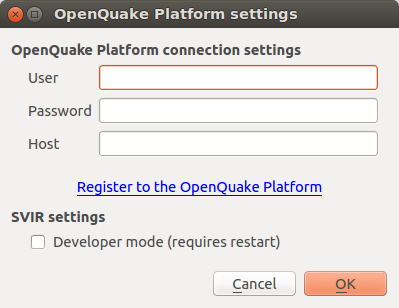
\includegraphics[width=0.8\textwidth]{../images/image07}
    \caption{OQ-Platform connection settings}
    \label{fig:connection_settings}
\end{figure}

Some of the functionalities provided by the plugin, such as the ability to work
with GEM data, require the interaction between the plugin itself and the
OpenQuake Platform (OQ-Platform). The OQ-Platform is a web-based portal to
visualize, explore and share GEM's datasets, tools and models. In the “Platform
Settings” dialog displayed in Figure~\ref{fig:connection_settings}, credentials
must be inserted to authenticate the user and to allow the user to log into the
OQ-Platform. In the ‘Host' field insert the URL of GEM's production
installation of the \href{https://platform.openquake.org}{OQ-Platform} or a
different installation if you have URL access. If you still haven't signed up
to the OQ-Platform, you can do so by clicking `Register to the OQ-Platform'.
This will open a new web browser and
\href{https://platform.openquake.org/account/signup/}{sign up page}.  The
checkbox labeled `Developer mode (requires restart)' can be used to increase
the verbosity of logging. The latter is useful for developers or advanced users
because logging is critical for troubleshooting, but it is not recommended for
standard users.

\section{Load socioeconomic indicators from the OpenQuake Platform}

\begin{figure}
    \centering
    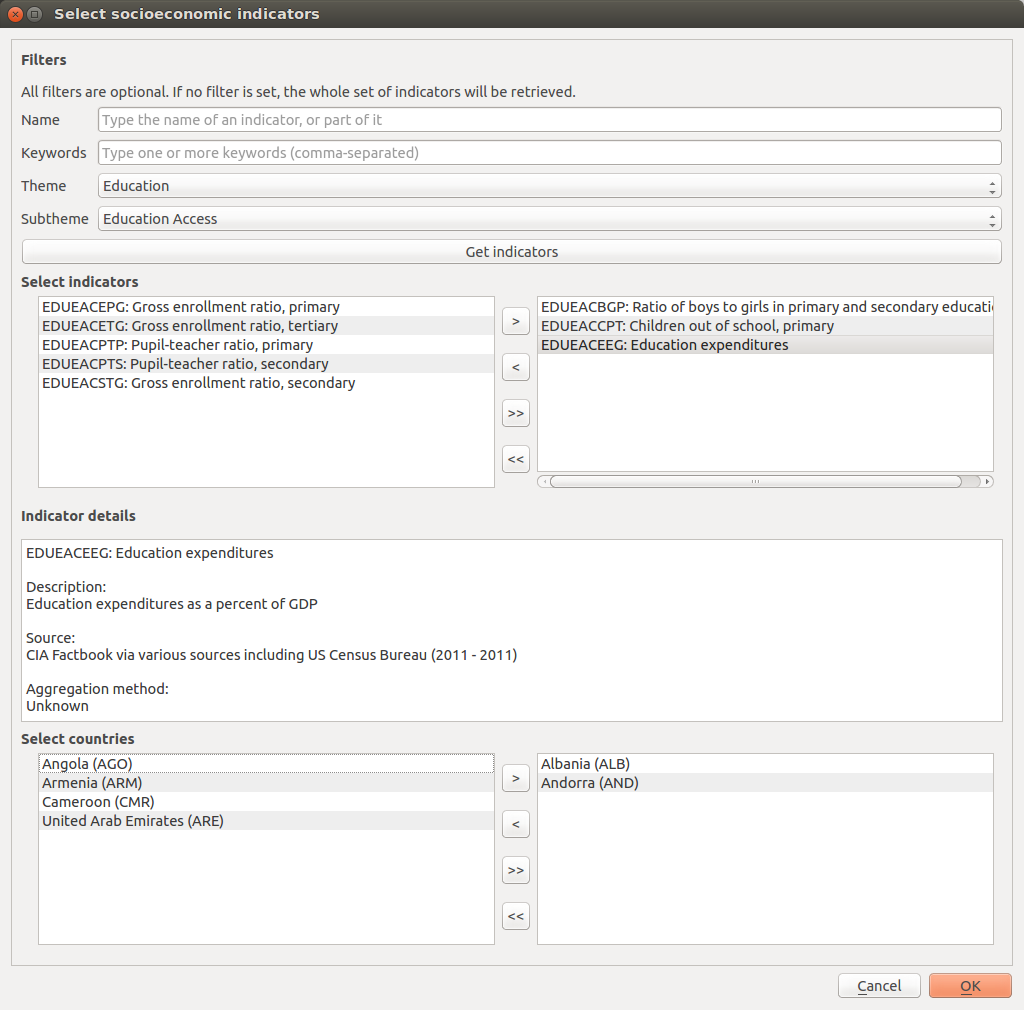
\includegraphics[width=\textwidth]{../images/image23}
    \caption{Socio-economic indicators selection portal}
    \label{fig:load_indicators_from_platform}
\end{figure}

The selection of data comprises an essential step for an assessment of risk
from an integrated and holistic perspective using indicators. The strengths and
weaknesses of composite indicators are derived to a great extent by the quality
of the underlying variables. Ideally, variables should be selected based on
their relevance to the phenomenon being measured, analytical soundness,
accessibility, and completeness\footnote{Nardo, M., Saisana, M., Saltelli, A.
and Tarantola, S. 2008. Handbook on constructing composite indicators:
Methodology and user guide. Paris, France: OECD Publishing}. Proxy measures for
social and economic vulnerability have been provided by the Global Earthquake
Model that have been stringently tested for representativeness, robustness,
coverage and analytical soundness\footnote{Khazai B, Burton C.G., Tormene, P.,
Power, C., Bernasocchi, M., Daniell, J., and Wyss, B. (2014). Integrated Risk
Modelling Toolkit and Database for Earthquake Risk Assessment. Proceedings of
the Second European Conference on Earthquake Engineering and Seismology,
European Association of Earthquake Engineering and European Seismological
Commission, Istanbul, Turkey}. These are currently accessible in the IRMT at
the national level of geography (gadm L1). Future software releases will add
access to data at gadm level 2 (L2) for a selection of countries and regions.
This will include the eight Andean countries of South America and countries
within Sub-Saharan Africa.

Figure~\ref{fig:load_indicators_from_platform}. displays the `Select
Socioeconomic Indicators' dialog that was developed to allow users to select
indicators based on a number of factors and filtering mechanisms. A
\emph{`Filters'} section was developed to enable users to filter indicators by
name, keywords, theme (e.g. Economy) and subtheme (e.g Resource Distribution
and Poverty). The `subtheme' dropdown menu is automatically populated depending
on the selection of a respective theme. When \emph{`Get indicators'} is
pressed, a list of filtered indicators is populated on the left side of the
dialog within the `Select indicators' window. If no filters are set, then the
whole list of indicators available within the database is retrieved and
displayed within the `Select indicators' window.

From the `Select indicators' window, it is possible to select one or more
indicators by single-clicking them in the `Unselected' list on the left.
Double-clicking the selected indicator(s) moves them to the `Selected' list on
the right, and the corresponding data will be downloaded from the OQ-Platform.
Another way to move items to the right, or back to the left, is to use the four
central buttons (`add the selected items', `remove the selected items', `add
all', `remove all'). The `Indicator details' section displays information about
the last selected indicator: code, short name, longer description, source and
aggregation method.

The `Select countries' dialog contains the list of enumeration types (in this
case countries) that socioeconomic data is available for within the database.
Countries can be selected from the list in the same manner that indicators are
selected using `Select indicators'. Once at least one indicator and one country
has been selected, the `OK' button will be enabled. By pressing the `OK'
button, data will be downloaded from the OQ-Platform and compiled into a vector
shapefile for display and manipulation within QGIS (another dialog will ask you
where to save the shapefile that will be obtained). The layer will contain
features equal to the number of selected countries and will contain all
attributes selected as indicators for the given countries. Additional
attributes will include fields containing country ISO codes and country names.
To reduce processing time, detailed country geometries were simplified using
ESRI's
\href{http://resources.arcgis.com/en/help/main/10.1/index.html#//007000000010000000}
{`Bend Simplify' algorithm}. Bend Simplify removes extraneous bends and small
intrusions and extrusions within an area's topology without destroying its
essential shape.

\begin{figure}
    \centering
    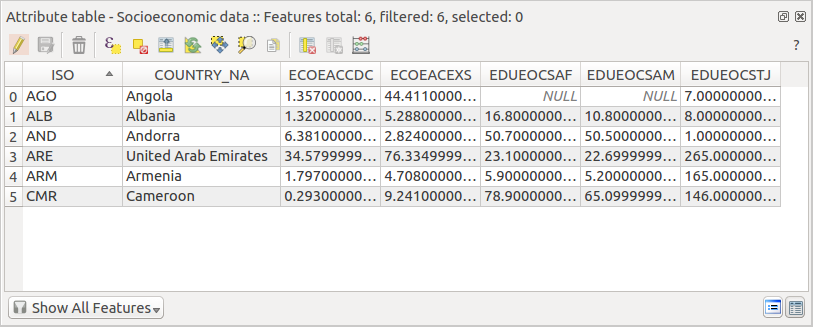
\includegraphics[width=\textwidth]{../images/image11}
    \caption{Layer attribute table}
    \label{fig:attribute_table}
\end{figure}

Figure~\ref{fig:attribute_table} shows the attribute table of a sample vector
layer compiled and downloaded within the IRMT\@. Note that for some countries the
values of indicators might be unavailable (or NULL). When the tool downloads
the socioeconomic data, a project definition is automatically built taking into
account how the data was organized in the socioeconomic database. At the
country level data was grouped together by these meaning that indicators
belonging to the same theme will be grouped together in a hierarchical
structure. This structure considers: 1) vulnerable populations; 2) economies;
3) education; 4) infrastructure; 5) health; 6) governance and institutional
capacities; and 7) the environment.

\section{Download project from the OpenQuake Platform}

\begin{figure}
    \centering
    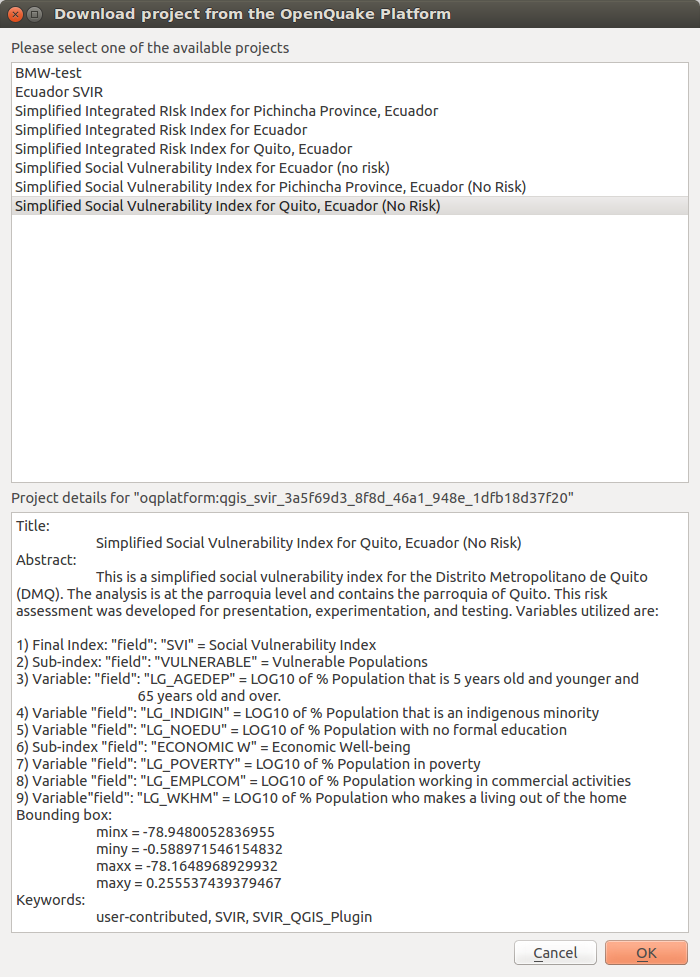
\includegraphics[width=\textwidth]{../images/image15}
    \caption{Download project from the OpenQuake Platform}
    \label{fig:download_project_from_platform}
\end{figure}

An additional option to access data is by downloading projects shared by others
on the OQ-Platform. By clicking the `Download project from the OpenQuake
Platform', the above dialog is opened (Figure 4). Here, a list of available
projects is displayed. The list will contain the titles of projects for which
the user has been granted editing privileges (their own projects or those
shared with them by other users). When a project is selected from the list, its
title, abstract, bounding box and keywords are displayed in the lower textbox
that is utilized to delineate important attributes of the project’s definition.
The label directly above the textbox displays an ID that uniquely identifies
the layer used in the OpenQuake-platform.

By pressing `OK', the layer will be downloaded into the QGIS\@. If the associated
project only contains one `project definition', it will be automatically be
selected and downloaded. Otherwise, the project definition manager will open
(see Section~\ref{sec:project_definitions_manager}) allowing the user to choose
one of the available project definitions. Once a project definition is
selected, the composite indicators delineated within the project definition are
re-calculated, and the layer is styled and rendered accordingly. This process
may take some time, depending on the complexity of the project.

\section{Transform attribute}

\begin{figure}
    \centering
    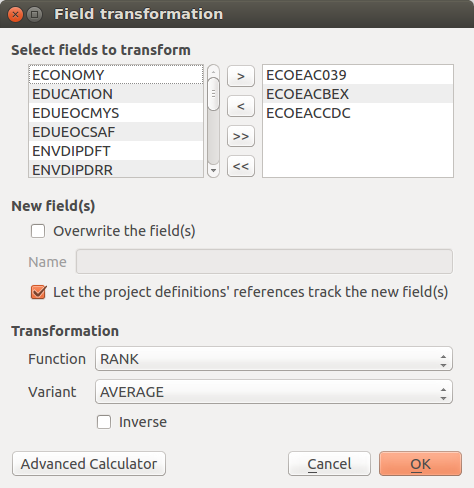
\includegraphics[width=\textwidth]{../images/image14}
    \caption{Variable transformation and batch transformation functionality}
    \label{fig:transform_attribute}
\end{figure}

Once variables are selected, they should be standardized or normalized before
they are aggregated into composite indicators. This is because variables are
delineated in a number of statistical units that could easily consist of
incommensurate ranges or scales. Variables are standardized to avoid problems
inherent when mixing measurement units, and normalization is employed to avoid
having extreme values dominate an indicator, and to partially correct for data
quality problems. The QGIS platform natively provides a `Field calculator' that
can be used to update existing fields, or to create new ones, in order to to
perform a wide variety of mathematical operations for the
standardization/transformation of data. In addition, the  IRMT provides a
number of transformation functions found in popular statistical and
mathematical modelling packages (Table~\ref{tab:transformation_functions}).

\begin{table}
\centering
\caption{Selection of transformation functions with equations found in the IRMT.}
\label{tab:transformation_functions}
\begin{tabular}{ll}
Standardization (or Z-scores) & $ Z(x_i) = \frac{x_i-\mu_x}{\sigma_x} $ \\
Min-Max & $ M(x_i) = \frac{x_i - \min_{i \in \{1,\dots,n\}}(x_i)}{\max_{i \in \{1,\dots,n\}}(x_i) - \min_{i \in \{1,\dots,n\}}(x_i)} $\\
Logistig Sigmoid & $ S(x_i) = \frac{1}{1 + e^{-x_i}} $ \\
Simple Quadratic & $ Q(x_i) = \frac{x^2}{\max_{i \in \{1,\dots,n\}}(x_i)} $
\end{tabular}
\end{table}

These include:
\begin{enumerate}
    \item \emph{Data Ranking} is the simplest standardization technique.
    Ranking is not affected by outliers and allows the performance of
    enumeration units to be benchmarked over time in terms of their relative
    positions (rankings).

    \item \emph{Z-scores (or normalization)} is the most common standardization
    technique.  A Z-score converts indicators to a common scale with a mean of
    zero and standard deviation of one. Indicators with outliers that are
    extreme values may have a greater effect on the composite indicator. The
    latter may not be desirable if the intention is to support compensability
    where a deficit in one variable can be offset (or compensated) by a surplus
    in another.

    \item \emph{Min-Max Transformation} is a type of transformation that
    rescales variables into an identical range between 0 and 1. Extreme
    values/or outliers could distort the transformed risk indicator. However,
    the MIN-MAX transformation can widen a range of indicators lying within a
    small interval, increasing the effect of the variable on the composite
    indicator more than the Z-scores.

    \item \emph{Log10} is one of a class of logarithmic transformations that
    include natural log, log2, log3, log4, etc. Within the current plugin, we
    offer functionality for log10 only, yet these transformations are possible
    within the advanced `field calculator'. A logarithm of any negative number
    or zero is undefined. It is not possible to log transform values within the
    plugin if the data contains negative values or a zero. For values of zero,
    the tool will warn users and suggest that a $1.0$ constant be added to move
    the minimum value of the distribution.

    \item \emph{Sigmoid function} is a transformation function having an ``S''
    shape (sigmoid curve). A Sigmoid function is used to transform values on
    $(-\infty, \infty)$ into numbers on $(0, 1)$.  The Sigmoid function is often
    utilized because the transformation is relative to a convergence upon an
    upper limit as defined by the S-curve. The IRMT utilizes a `simple sigmoid
    function' as well as its inverse. The Inverse of the Sigmoid function is a
    logit function which transfers variables on $(0, 1)$ into a new variable on
    $(-\infty, \infty)$.

    \item \emph{Quadratic or U-shaped functions} are the product of a
    polynomial equation of degree 2. In a quadratic function, the variable is
    always squared resulting in a parabola or U-shaped curve. The IRMT offers
    an increasing or decreasing variant of the quadratic equation for
    horizontal translations and the respective inverses of the two for vertical
    translations.
\end{enumerate}

Please note that it may be desirable to visualize the results of the
application of transformation functions to data. Although not feasible within
the plugin at this point, we intend to build data plotting and curve
manipulating functionalities into into future versions of the toolkit.   

The `Transform attribute' dialog (Figure~\ref{fig:transform_attribute}) was
designed to be quite straightforward. The user is required to select one or
more numeric fields (variables) available in the active layer. For the
selection to be completed, the user must move the variables (either one at a
time, or in a batch) to the `Selected variables' window on the right side of
the interface. The user must then select the function necessary to transform
the selected variables. For some functions, more than one variant is available.
For functions that have an implementation of an inverse transformation, the
`Inverse' checkbox will be enabled to allow users to invert the outcome of the
transformation.

The `New field(s)' section contains two checkboxes and a text field. If the
first checkbox `Overwrite the field(s)' is selected, the original values of the
transformed fields will be overwritten by the results of the calculations;
otherwise, a new field for each transformed variable will be created to store
the results. In situations in which a user may desire to transform variables
one at a time rather than using a batch transformation process, it is possible
for the user to name each respective new field (editing the default one
proposed by the tool). Otherwise, the names of the new fields will be
automatically assigned using the following convention: if the original
attribute is named `ORIG\_NAME', the name of the transformed attribute becomes
`T\_ORIG\_NAM' (prepending `T\_' and truncating to 10 characters which is the
maximum length permitted for field names in shapefiles).

If the checkbox `Let the project definitions' references track the new
field(s)' is checked, all the project definitions associated with the active
layer will reference the transformed fields instead of the original ones.
Otherwise, they will keep the links to the original selected attributes. In
most cases it is recommended to keep this checkbox checked. This automatic
update of field references simplifies the workflow because it avoids the need
to manually remove the original nodes from the weighting and aggregation tree
(discussed in detail in Section~\ref{sec:weighting_and_calculating}) in
order to add the transformed nodes and to set again the nodes' weights. In
other words, if a project was developed by weighting and aggregating
untransformed indicators, this functionality allows for variables used in the
project definition to be replaced on-the-fly (and automatically) by transformed
variables.  This saves the user from having to augment the model manually.  

By clicking the `Advanced Calculator' button, the native QGIS field calculator
is opened.  Please refer to
\url{https://github.com/gem/oq-svir-qgis/blob/master/transformation_algs.py}
for the detailed documentation of all the agorithms and variants provided by
the IRMT.


\chapter{Project definitions manager}
\label{chap:project_definitions_manager}

\begin{figure}
    \centering
    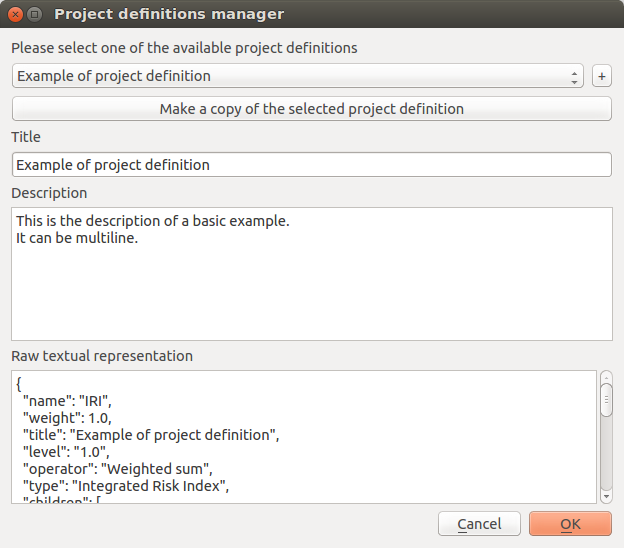
\includegraphics[width=\textwidth]{../images/image13}
    \caption{Project definitions manager}
    \label{fig:project_definitions_manager}
\end{figure}

The `Project Definitions Manager' is a module that was developed to allow users
to create multiple models that can be accessed with a click of a button using a
single layer. Each `project definition' (see Chapter~\ref{chap:definitions}) can
define a different model structure, weighting and aggregation scheme, and
variable selections among data available in the underlying layer. It allows
users to seamlessly toggle through various integrated risk assessment projects
without having to refer to different `QGIS projects' or different `layers'
containing data for a given area or areas, and without having to re-symbolize
data to compare results of assessments using different methodological
parameters. The `Project definitions manager' was developed around a dialog
window that enables users to edit the current project definition, to switch
from the current project definition to a different one, to add a new project
definition, or to clone an existing project definition.

While contributing to the `Title' and `Description' textbox of the project
definitions manager, the `Raw textual representation' is updated accordingly.
Please note that it is not recommended for users to edit the parameters
directly inside the `raw textual representation' portion of the project
definition manager, although it is not forbidden. This especially applies to
variable names (field names) and sub-indicators (also field names) defined by
nodes within the weighting and aggregation tree (see
Chapter~\ref{chap:weighting_and_calculating}). Manual adjustments can be useful
in some corner cases, by experienced users, but manual adjustments can cause
the toolkit to behave unexpectedly and can cause shapefiles to behave
unexpectedly. Users performing these adjustments are at risk of compromise
their data.

The `+' button at the right of the dropdown menu can be used to associate the
current layer with a new project definition. By clicking it, a new basic
project definition is created and the user is invited to provide the new
project definition with a title and, possibly, a description.  The button `Make
a copy of the selected project definition', assigns to the active layer within
the QGIS a new project definition that is an exact clone of the selected one.
Having two similar project definitions can be useful to easily visualize how
the output of a project is changed based on  updated variable selections,
weighting, and aggregation schemes. This visualization is possible because a
simple click is sufficient to switch between `before' and `after' project
definitions. When `OK' is pressed, the composite indices are re-calculated
accordingly with the project definition and the layer is styled as a
consequence via a default classification and symbolization that is adjustable
within the QGIS\@. This computation can take some time, depending on the
complexity of the layer.

\chapter{Weighting data and calculating indices}
\label{chap:weighting_and_calculating}

\begin{figure}
    \centering
    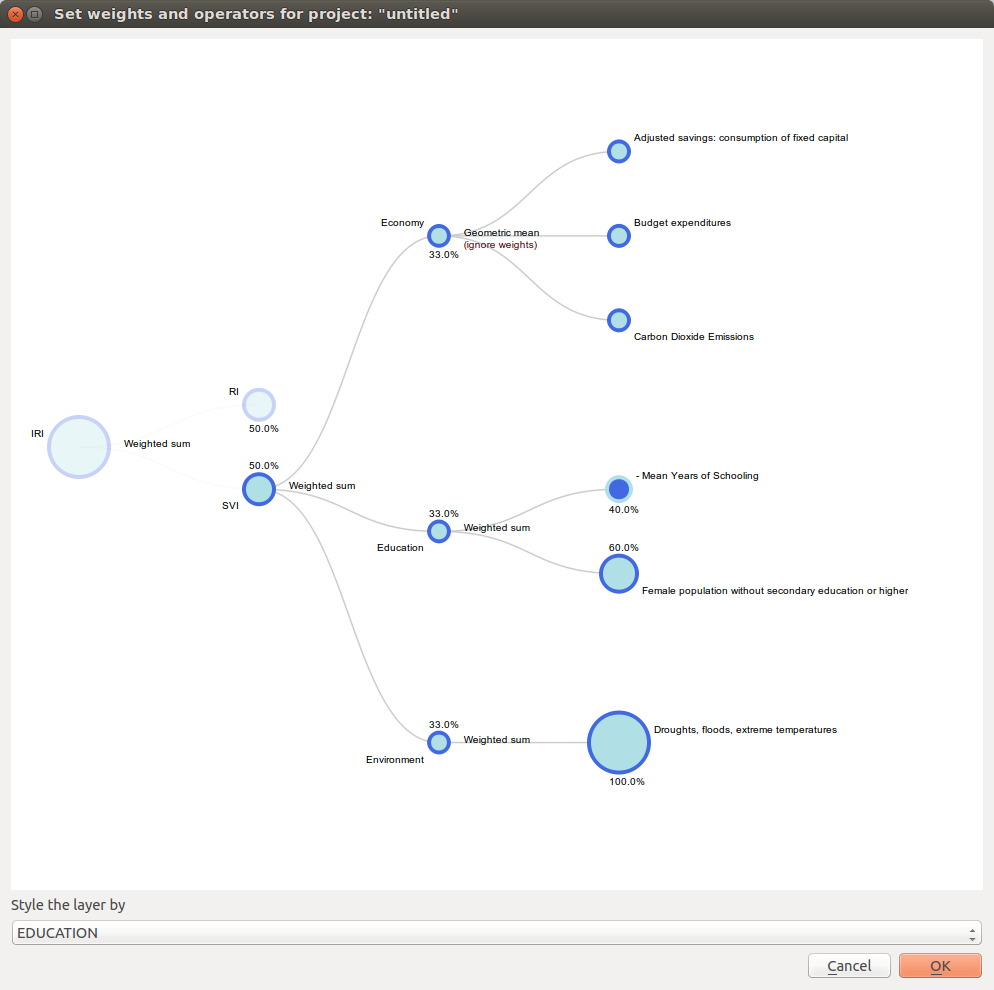
\includegraphics[width=\textwidth]{../images/image06}
    \caption{Tree chart structure for the development of composite indicators}
    \label{fig:weighting_and_calculating}
\end{figure}

Central to the construction of composite indicators is the need to meaningfully
combine different data dimensions, and consideration must be given to weighting
and aggregation procedures. Most composite indicators rely on equal weighting
largely for simplicity. Equal weighting, however, implies that all variables
within the composite indicator are of equal importance when this may not
actually be the case. The issue of aggregation is similar to the weighting
process. Different aggregation rules may be applied depending on the underlying
theoretical framework chosen by the user for the modelling process.
Sub-indicators may be summed up (linear aggregation) for instance, multiplied,
or geometrically aggregated to correct for compensability (i.e.\ the possibility
of offsetting a deficit in some dimension with an outstanding performance in
another). Each technique has specific consequences, implies different
assumptions, and could ignore or incorporate weights.

The `Weight data and calculate indices' application
(Figure~\ref{fig:weighting_and_calculating}) is the key module of the IMRT\@. It
contains the model building functionality of the IRMT, and it is used to
create, edit, and manage composite indicator(s) and integrated risk model
development. The `Weight data and calculate indices' application provides users
with an intuitive way to develop composite models by building and editing the
selected project definition through the use of a dynamic graphical interface
that was developed explicitly to guide the construction of composite indicators
in a manner that is simple, visual, and straight-forward. The latter is
accomplished through a window that embeds a web browser in which a javascript
D3 tree chart is rendered (see Figure~\ref{fig:weighting_and_calculating}).
This tree chart structure (or weighting and aggregation tree) defines a
workflow that strings together sequences of steps to describe how variables are
combined together to obtain the composite indices.  

\begin{figure}
    \centering
    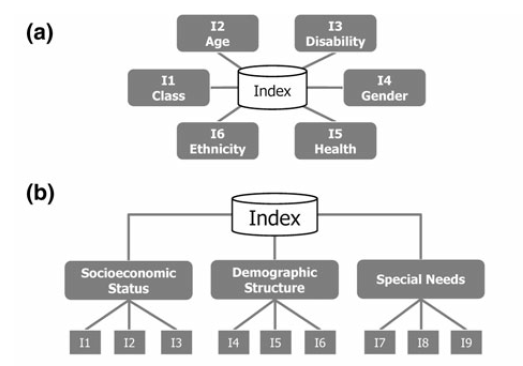
\includegraphics[width=\textwidth]{../images/image19}
    \caption{Composite indicator types (adapted from: Tate, E.C. 2012.
    Social vulnerability indices: a comparative assessment using uncertainty
    and sensitivity analysis, Natural Hazards, 63(2): 325-347)}
    \label{fig:composite_indicator_types}
\end{figure}

Currently, the IRMT supports the development of two composite model types: a)
deductive and, b) hierarchical (Figure~\ref{fig:composite_indicator_types}).
Deductive models typically contain fewer than ten indicators that are
normalized and aggregated to create an index. Hierarchical models typically
employ ten to twenty indicators that are separated into groups (sub-indices)
that share the same underlying dimension of a concept (in this case
socio-economic parameters of earthquake risk such as population, economy,
infrastructure, education, and governance).  Individual indicators are
aggregated into sub-indices (e.g.\ population, economy, etc), and the
sub-indices are aggregated to form a final composite index (e.g.\ a social
vulnerability or integrated risk index). The tree structure of the `Weight data
and calculate indices' application encourages the development of hierarchical
models of integrated risk. The starting point is a `root node' that corresponds
to the development of a hierarchical model that can be: 1) an `Integrated Risk
Index' (IRI) which is a function of the aggregation of a `Social Vulnerability
Index' (SVI) and a `Risk Index' (RI); or 2) a `Social Vulnerability Index'
(SVI) that is the result of the aggregation of various sub-indicators defined
by the user (e.g.\ Economy, Education, and Environment as shown within
Figure~\ref{fig:weighting_and_calculating}).  The tree can be modified
dynamically by adding or removing nodes, `inverting' variables, setting a
weight to each variable or node and choosing the operators to be used to
combine variables together.

Whenever `Update' or `Update and close' are clicked, the project definition is
updated and the composite indices are re-calculated. As a consequence, the map
is rendered and styled accordingly. This allows the user to have an immediate
feedback on how the map changes depending on how the project definition is set.
Such automatic re-calculations and rendering can take some time, depending on
the complexity of the project and number of enumerations units analysed.

The main functional elements of the weighting and aggregation tree are
discussed in the subsections below.


\section{Adding a node}

Individual nodes correspond to aggregated composite indicators within the
weighting and aggregation tree. To add a node (i.e.\ a composite sub-indicator)
within the tree, it is possible to begin by left-clicking on the default node
(i.e.\ SVI).  Clicking on the default SVI node allows the addition of multiple
new sub-indicators, each with its own user-provided name (note that it is not
possible to add nodes stemming from the IRI). When a newly created node is
clicked, a new dialog is initiated to give users the option to select the
variables available in the layer (and not already used in the node) to populate
the sub-indicator being under construction. Please note that the SVI can be
calculated if each socioeconomic sub-indicator has at least one variable. In
order to add an indicator to one of the socioeconomic sub-indicators, you can
click on the corresponding node. When adding an indicator to the RI, or to one
of the socioeconomic sub-indicators, the description of the node will be
automatically set to be equal to the name of the corresponding layer's
variable. Users can edit this description, however, by clicking on the text
displayed next to the node in the tree and then by clicking within the
corresponding textbox to change the text.


\section{Removing a node}

In order to remove one of the nodes from the tree, users can perform a
right-click on that node. A popup dialog window will ask you to confirm if you
really intend to delete the node and all of its `children' (the lower level
nodes connected to it). Please note that removing a node from the tree will not
delete the corresponding field from the layer.


\section{Setting the operators to be used to combine nodes together
(variable aggregation)}
\label{sec:setting_operators}

On the right of each node, the tree indicates the name of the operator to be
used to combine (or aggregate) the `children' of such node. By clicking on the
operator's name, a dialog to set weights and operators is opened. The same
happens when clicking on the name of one of the children nodes. The operator
can be chosen from a dropdown menu. Some operators (e.g., `Weighted sum') take
into account the weights applied to the child nodes. Other operators (e.g.,
`Average (ignore weights)') do not take into account weights. When the chosen
operator is one of the latter, the child nodes will be rendered on the
graphical display all with the same radius and their weights will not be
rendered (see Figure~\ref{fig:weighting_and_calculating} for a demonstration of
how the radius of nodes corresponds with the respective weights of variables).
Otherwise, the radius of a node is proportional to its weight, and the weight
is rendered next to the node.


\section{Setting weights}

Central to the construction of composite indicators in the need to combine data
into meaningful dimensions which implies decisions on weighting. The dialog to
set weights is opened in the same way as described in
Section~\ref{sec:setting_operators}. Several weighting techniques are
available, and some make use of statistical models.  For the IRMT we
implemented a simple solution to weighting that is often based on the results
of participatory approaches. A weight can be edited manually by clicking on its
value and overwriting it with a new value. A weight can also be edited by
clicking on the spinner's arrows to increase or decrease the weight.  By
clicking `Update', the weights will be re-calculated in order to make them sum
to 1. In other words, if you have 3 variables and you set their weights to 1, 2
and 5 and you press `Update', the weights will be re-calculated to be
respectively 0.125, 0.250 and 0.625, keeping the same proportion between each
other, and summing to 1.


\section{Inverting a variable}

The dialog to invert variables is opened in the same way as described in
Section~\ref{sec:setting_operators}. If a variable contributes in a `negative'
way to the composite indicator (e.g., a higher education corresponding to a
lower social vulnerability), it is possible to indicate such an inverse
relationship by pressing the `Invert' button next to the variable name. The
effect on a composite indicator in response to this decision process and
setting is that each value of the `inverted' variables will be to multiplied by
-1 each time the variables themselves are used in a calculation.  Please note
that the layer's field will keep holding the original value of the variable,
and that the inversion will be performed on-the-fly for the purpose of the
calculation.


\section{Assigning a new name to a variable}

The dialog to assign a new name to a variable is also opened in the same way as
described in Section~\ref{sec:setting_operators}. By clicking on the variable's
name, a popup dialog asks users to insert the new name. The project definition
will be updated accordingly, linking the layer's fieldname with the modified
description.


\section{Styling the layer by a chosen field}

The dropdown menu on the bottom of the `Set weights and operators' module can
be used to choose fields within a layer, i.e., fields other than those
delineated within the project definition to be symbolized, allowing all fields
in a layer to be to be symbolized on-the-fly.  This can be useful, for
instance, to map the values calculated for different sub-indicators, or even
individual variables if they are of interest. By default, the selection is
blank. In the default case, the tool will adopt the following convention: 1) if
the IRI can be computed, then the layer will be symbolized according to it; 2)
otherwise, if the SVI can be computed, then it will be used as the default case
for symbolization in the absence of IRI; 3) otherwise, the convention will
apply with respect to the RI; and 4) if none of main sub-indicators can be
calculated, then the layer will not be re-styled unless the user uses the
dropdown menu to specify a specific symbolization field.

\section{Aggregate loss by zone}

\begin{figure}
    \centering
    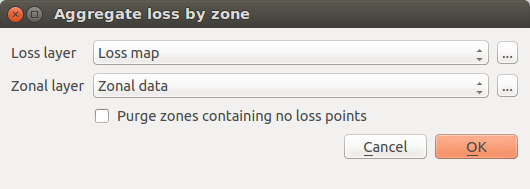
\includegraphics[width=\textwidth]{../images/image08}
    \caption{`Aggregate loss by zone' data import tool}
    \label{fig:aggregate_loss_by_zone}
\end{figure}

The development of an integrated risk model (IRI) arises from the convolution
of two main components: 1) estimations of physical risk (RI), and 2) a social
vulnerability index (SVI). The convolution of earthquake physical risk and
social vulnerability parameters can be accomplished by, first, importing risk
assessments from OpenQuake (or some other source) using the toolkit's risk
import tool (Figure~\ref{fig:aggregate_loss_by_zone}). As a subsequent step,
earthquake risk data imported into the tool should be standardized to render
the data commensurate to the socioeconomic indicators created within the tool.

To import data, users can click the `Aggregate loss by zone' button which
prompts a dialog window to open. Here, it is possible to select layers
containing estimations of physical risk, (`Loss layer') or some other type of
risk model, and to combine these with a layer containing zonal geometries of
the study area (e.g.\ country borders, district borders) and socioeconomic
indicators. The top dropdown menu is pre-populated with the names of the
available vector layers containing point geometries (a native output of the
OQ-Engine), while the second dropdown menu is pre-populated with the names of
the available vector layers containing polygonal geometries. If those menus do
not contain the desired layers, it is possible to click one of the `\dots'
buttons, to load another layer from the file system. As soon as a new layer is
loaded, it will be available in the QGIS table of contents and its name will
become available and pre-selected in the corresponding dropdown menu.

Estimations of physical risk can be made available from the OQ-Engine as one or
multiple CSV files. By selecting the file type `Loss curves from the
OpenQuake-engine', such files become available and can be (multi)selected. The
resulting loss layer will contain a number of attributes equal to the number of
CSV files imported, and each attribute will correspond to a different loss
type.


\begin{figure}
    \centering
    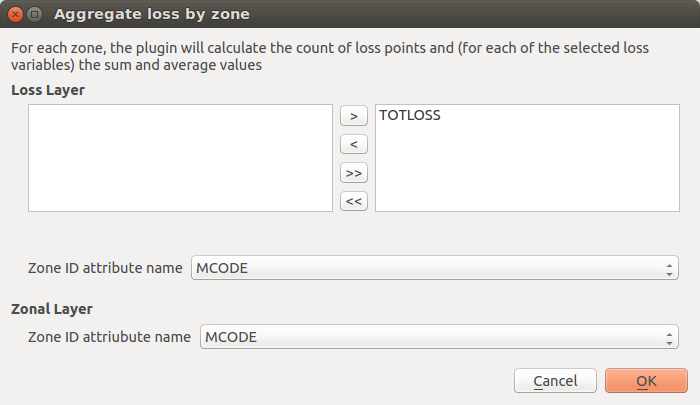
\includegraphics[width=\textwidth]{../images/image09}
    \caption{Zonal aggregation of loss values}
    \label{fig:zonal_aggregation_of_loss_values}
\end{figure}

Loss data from the OQ-Engine is rendered as points containing X,Y locational
coordinates and the loss values for the different assets represented at a given
location. Once both a loss layer and a zonal layer have been selected, the
above dialog window is opened
(Figure~\ref{fig:zonal_aggregation_of_loss_values}). In the `Loss Layer'
section of the dialog window, the user is invited to select one or more
attributes from the loss layer. This selection is because the toolkit will
calculate the sum and average values for each of the zonal layer's features,
and it will add those statistics to the zonal layer as new attributes. Within
the layer's attribute table, a subsequent attribute will be added to display
the count of loss points that are found inside the boundaries of each feature.
The latter can be useful for troubleshooting.

The `aggregation by zone' can be obtained in different ways. If the user is
aware that both the loss layer and the zonal layer contain a common attribute
that indicates the id of the zone to which each feature belongs, then it is
sufficient to select this common attribute both for the loss layer and the
zonal layer, and let the tool perform a simple join. In this case, the
aggregation is fast because it does not require spatial analysis.

If a common zonal ID does not exist, a spatial join using zonal geometries may
be utilized. This is accomplished, first, by selecting `Use zonal geometries'
within the `Zone ID attribute name' dropdown menu that contains also the names
of all the attributes of the loss layer. As a consequence, the tool will
perform a spatial search to detect to which zone each of the loss points
belongs. The `Zone ID attribute name' in the zonal layer is the attribute that
uniquely identifies each of the zones. If the user is not sure if features are
uniquely identified by any of the available attributes in the zonal layer, then
it is possible to select the additional item `Add field with unique zone id'.
As a consequence of this choice, the tool will produce an additional attribute
in the corresponding layer, and it will set the values of that attribute to be
equal to the unique id of the corresponding feature. Then the new attribute
will be used as unique id of the feature, to perform the loss aggregation by
zone.

\chapter{Upload project to the OpenQuake Platform}

\begin{figure}
    \centering
    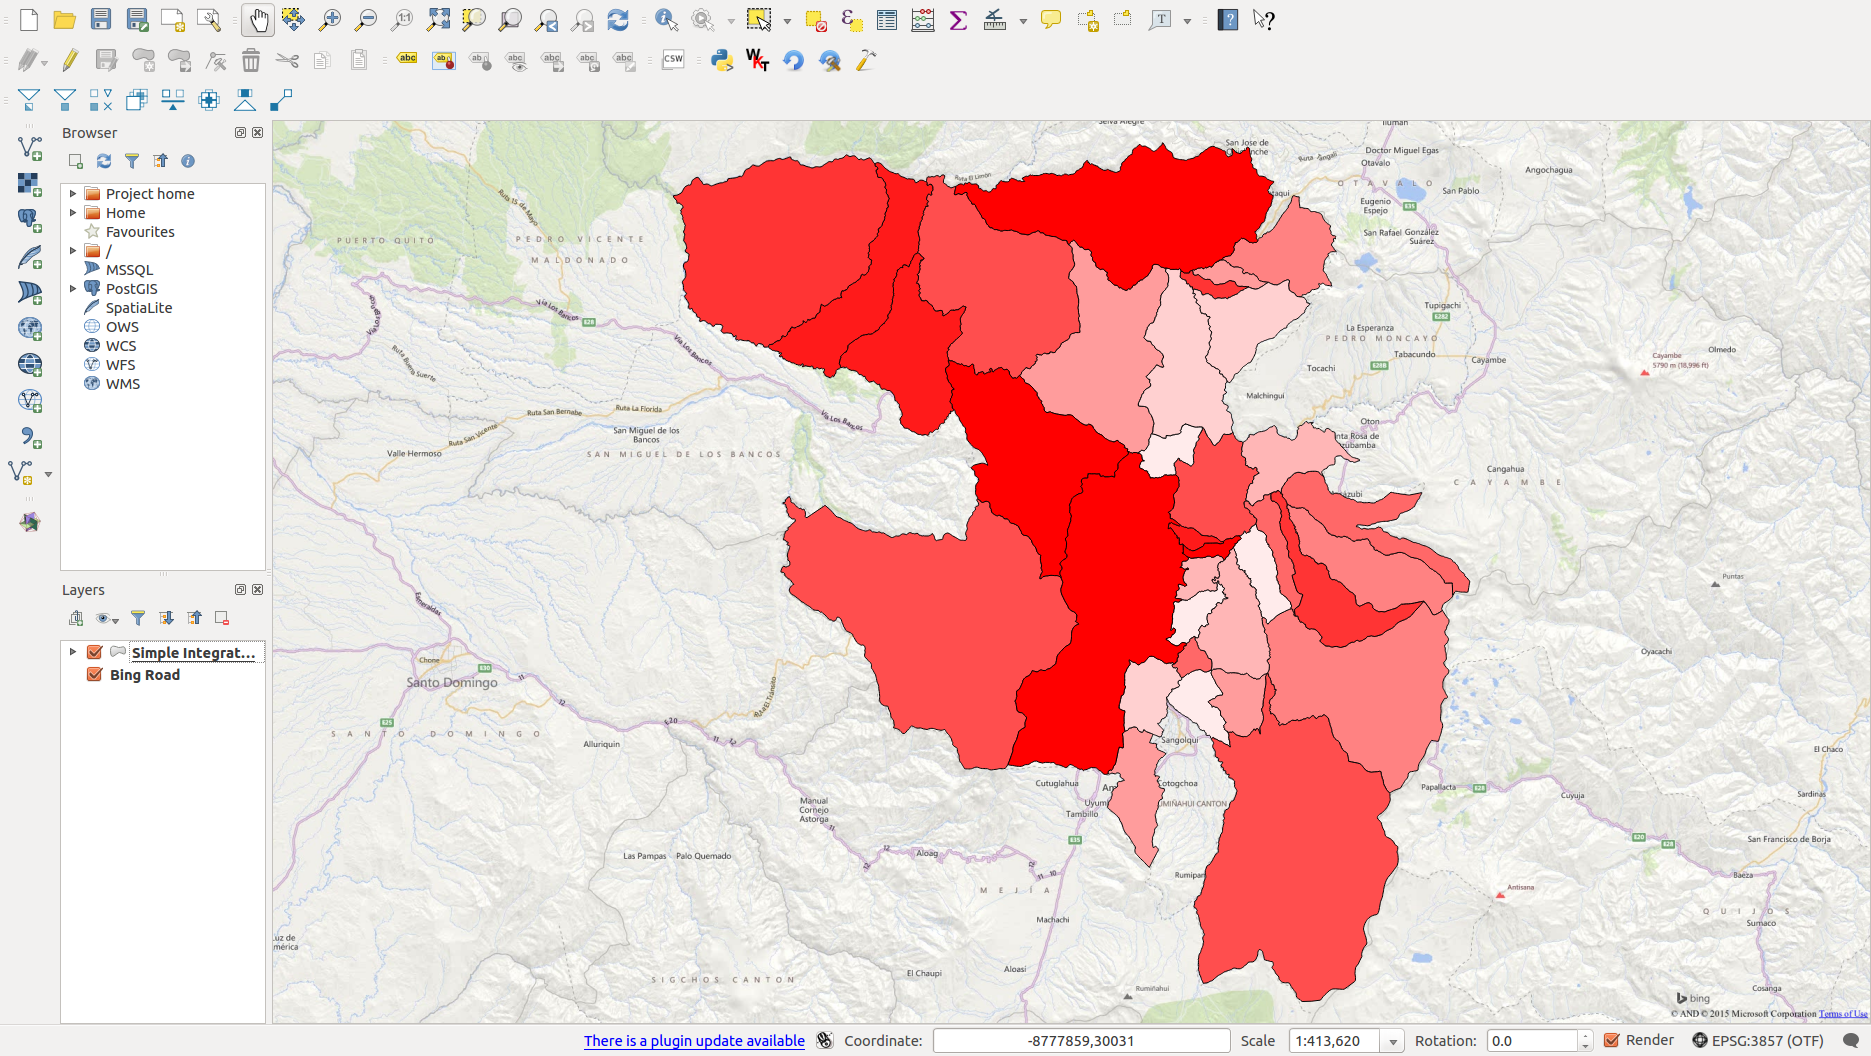
\includegraphics[width=\textwidth]{../images/image22}
    \caption{Simplified Integrated Risk analysis as it is seen inside QGIS
    right before the project is uploaded to the OpenQuake Platform}
    \label{fig:before_uploading}
\end{figure}

Once an integrated risk model is complete, and the user is satisfied with
results such as those obtained for the example displayed in
Figure~\ref{fig:before_uploading}, it is possible to upload projects through
the OQ-Platform. Projects are uploaded in order to share them with the wider
earthquake risk assessment, earthquake risk reduction, GIS communities, etc.
Uploading to the OQ-Platform also  supports the ability to visualize models
using advanced visualization tools and the mapping of the data over the web. In
addition, sharing the models on the OQ-Platform allows users that are not QGIS
savvy to dynamically interact with the data. The mapping and visualization over
the web is accomplished using the OQ-Platform
(Figure~\ref{fig:after_uploading}) and the Social Vulnerability and Integrated
Risk Viewer (the web application is available at
\url{http://www.globalquakemodel.org/openquake/support/documentation/platform/irv/}
and the corresponding documentation can be found at
\url{https://platform.openquake.org/irv_viewer/}).

\begin{figure}
    \centering
    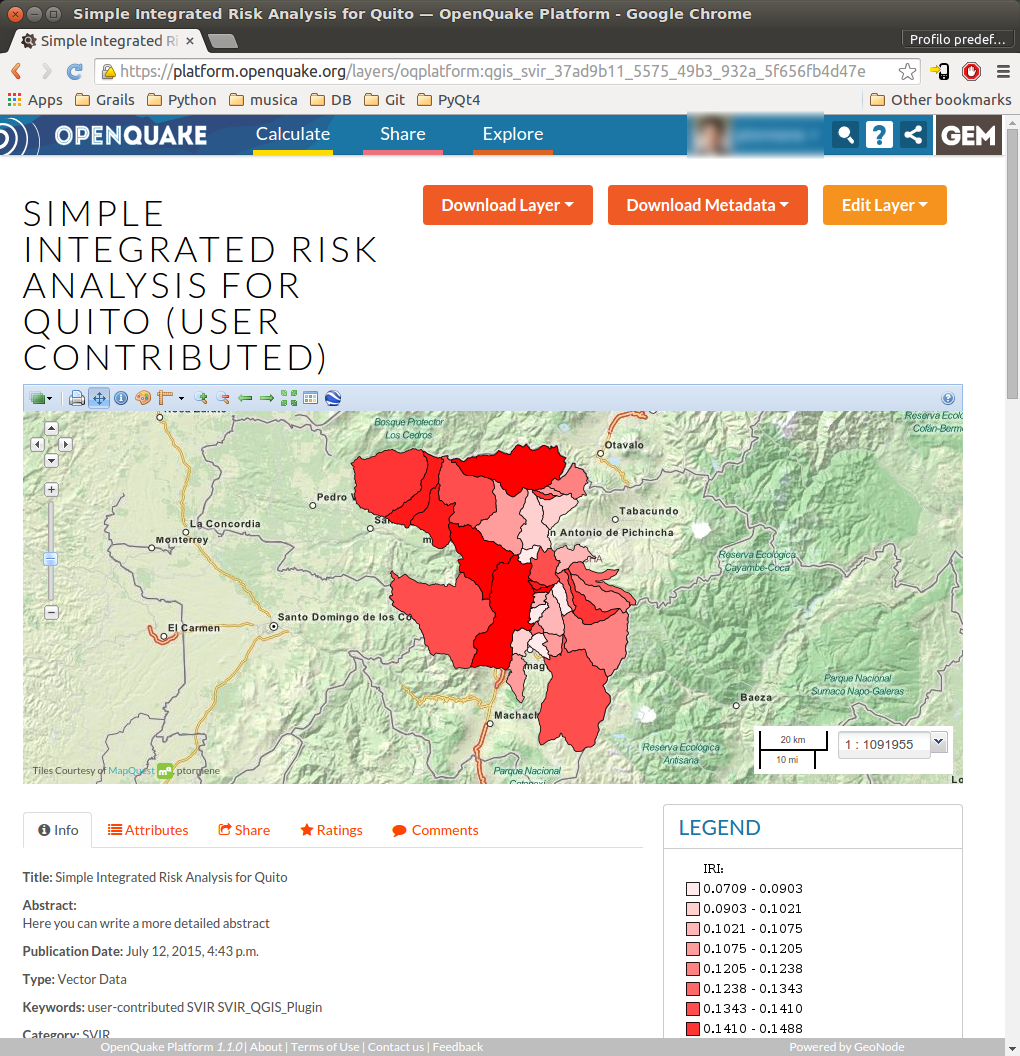
\includegraphics[width=\textwidth]{../images/image10}
    \caption{The same simple example shown in
    Figure~\ref{fig:before_uploading}, visualized through a web browser after
    it has been uploaded to the OpenQuake Platform}
    \label{fig:after_uploading}
\end{figure}

To upload a project to the OQ-Platform, click `Upload project to the OpenQuake
Platform'. This will result in the opening of a dialog window in which,
depending on the context, the window will look like those delineated in
Figure~\ref{fig:upload_dialog} or~\ref{fig:update_dialog} 13 or 14. The former
will be displayed if the current project has never been uploaded to the
OQ-Platform. In such cases, the user is invited to provide a project title that
will become the title of the Geonode layer that will be created on the
Platform. A second field will contain the abstract, where the user can provide
a general description of the project.

\begin{figure}
    \centering
    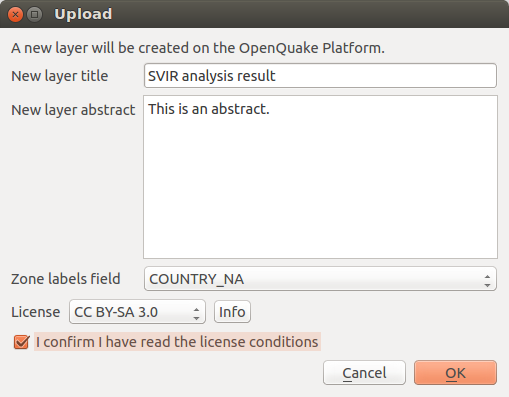
\includegraphics[width=\textwidth]{../images/image25}
    \caption{Uploading a project to the OpenQuake Platform}
    \label{fig:upload_dialog}
\end{figure}

In order to be able to correctly utilize the advanced visualization tools found
on the OQ-Platform, the selection of a `Zone labels field' is required (see
Figure~\ref{fig:upload_dialog}). The user must designate the `Zone labels
field' within their dataset. The latter is a field containing unique labels (or
identifiers) whether these be individual country names, district names, or
census block numbers. Delineating a zone field when uploading to the
OQ-Platform is imperative to allow the graphing components of the Social
Vulnerability and Integrated Risk Viewer to render the visualization using the
zone's labels.  Without the latter, comparisons among places within the
graphing tools are not possible. It is also mandatory to choose a license and
to click on the checkbox to confirm to be informed about the license
conditions. By clicking the `Info' button, a web browser will be opened,
pointing to a page that describes the license selected in the `License'
dropdown menu. When `OK' is pressed, the active layer is uploaded to the
OQ-Platform and it is applied in the same style visible in QGIS\@. Furthermore,
the current project definition is saved into the Geonode layer's metadata,
inside the `Supplemental information' field.

\begin{figure}
    \centering
    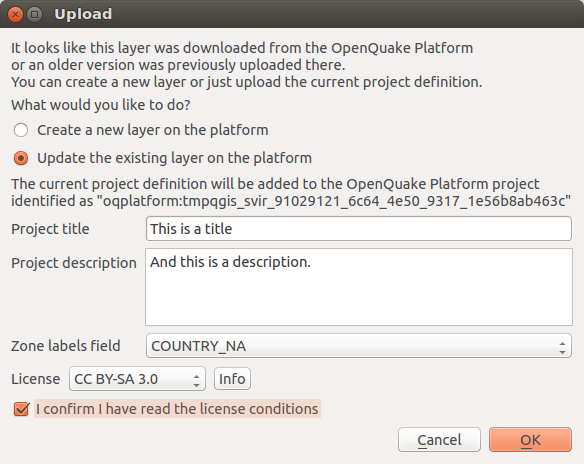
\includegraphics[width=\textwidth]{../images/image21}
    \caption{Updating a project that has already been uploaded to the OpenQuake Platform}
    \label{fig:update_dialog}
\end{figure}

This second version of the `Upload' dialog window is displayed when the active
layer appears to have been already shared through the OQ-Platform (the ID of a
OQ-Platform's layer was previously associated with this layer). In such cases,
it is possible to create a brand new layer, ignoring the previously uploaded
(or downloaded) project, or to update the current layer. The updating process
consists of adding the current project definition to the set of project
definitions associated to that layer on the OQ-Platform. This is a much faster
procedure because no geometries need to be uploaded, and only the metadata of
the Geonode layer will be changed.


% %----------------------------------------------------------------------------------------
% %	BIBLIOGRAPHY
% %----------------------------------------------------------------------------------------
% \chapter*{Bibliography}
% \addcontentsline{toc}{chapter}{\textcolor{ocre}{Bibliography}}
% \section*{Books}
% \addcontentsline{toc}{section}{Books}
% \printbibliography[heading=bibempty,type=book]
% \section*{Articles}
% \addcontentsline{toc}{section}{Articles}
% \printbibliography[heading=bibempty,type=article]
% \section*{Other Sources}
% \addcontentsline{toc}{section}{Reports}
% \printbibliography[heading=bibempty,nottype=book,nottype=article]


% %----------------------------------------------------------------------------------------
% %	INDEX
% %----------------------------------------------------------------------------------------

% \cleardoublepage
% \phantomsection
% \setlength{\columnsep}{0.75cm}
% \addcontentsline{toc}{chapter}{\textcolor{ocre}{Index}}
% \printindex
% \printglossary

% %----------------------------------------------------------------------------------------


% \part{Appendices}
% \appendix
% % -----------------------------------------------------------------------------
% % -----------------------------------------------------------------------------
% \chapter{The 10 Minute Guide to Python!}
% \label{sec:python_guide}
% %\begin{myfancybox}
% % The objectives of this chapter are:
% %\begin{itemize}
% %     \item To introduce Python data types to facilitate use of the HMTK for Python beginners
% % \end{itemize}
% %\end{myfancybox}
% \input{python_guide.tex}


\end{document}

